%!TEX root = ../thesis.tex

\thispagestyle{myheadings}
\graphicspath{{Body/Figures/Theory/}}

\chapter{Introduction}
\label{chapter:Introduction}

The prevailing theory for particle physics, the Standard Model (SM), has had tremendous success in describing our universe. It has been used to predict and explain a wide variety of phenomena, particles, properties, and interactions to great precision. However, in spite of its success in explaining nearly all experimental results, there remain unanswered questions about our universe. Some of these include the matter-antimatter asymmetry, the source of mass for the neutrinos, the existence of dark matter, and an inability to fully incorporate our best theory of gravitation. Many particle physics experiments around the world are being devised and conducted in order to shed light on these questions and improve our understanding of reality. One such particular experiment is the Fermilab Muon \gmtwo Experiment (E989) underway at the Fermi National Accelerator Laboratory (FNAL) located in Batavia, Illinois.

I have been a part of the E989 experiment since I began my graduate degree six years ago. Three years ago I moved from Boston to Batavia to get more involved by being where the action is. This dissertation will describe the E989 experiment and the work which I have done for it along the way in detail. Chapter 1 will provide experimental and theoretical background to the experiment, as well its motivation. Chapter 2 will describe the experimental principle. Chapter 3 will describe the magnetic field portion of the experiment, and magnetic field simulations I conducted. Chapter 4 will describe the straw tracking detectors and their measurements, including the track fitting I wrote. Chapter 5 will describe the frequency measurement portion of the experiment, and detail my analysis results from data taken in the first half of 2018. Finally, Chapter 6 will concluded the thesis and the results contained within.


\section{Magnetic Moments of Particles}
\label{sec:MDMs}

In order to understand the purpose of the Fermilab Muon \gmtwo Experiment, first we need to understand what the $g$ in \gmtwo is. This is what the experiment is measuring. All particles have intrinsic properties. One of those properties is the magnetic dipole moment.\footnote{\textit{Magnetic dipole moment} and \textit{magnetic moment} are equivalent when talking about particles.} This property of a particle is related to its spin through the equation
		\begin{align}
            \vec{\mu} = g \frac{q}{2m} \vec{s},
        \label{eq:magneticmoment}
		\end{align}
where $\vec{\mu}$ is the magnetic dipole moment of a particle, $\vec{s}$ is its spin vector, $m$ is its mass, $q = \pm e$ where $e$ is the elementary charge, and \g is the so called "g-factor". \g is some measureable and predictable constant, which as shown in \equref{eq:magneticmoment} relates the magnetic moment of a particle to its spin angular momentum. Since the torque on a particle in a magnetic field is 
		\begin{align}
            \vec{N} = \vec{\mu} \times \vec{B},
        \label{eq:torque}
		\end{align}
the rate at which a particles spin precesses in a magnetic field will depend on \g. This happens to be one of the key physics principles in the E989 experiment as will be discussed later.

In a Dirac theory, \g is equal to 2 for spin-1/2 particles with no internal structure \cite{Dirac}. See Appendix~\ref{gDirac} for a nice derivation of this result. It turns out however, that \g is not quite equal to 2 even for these types of particles. Motivated by early experimental discrepencies such as the measurements of the hyperfine structure in hydrogen \cite{EarlyHyperfine1}, in 1948 Schwinger calculated the first "radiative correction" to the electron magnetic moment \cite{Schwinger}. In a quantum field theory, interactions of the particle with virtual particles in loops will contribute to the value of \g. In this context it is nicer to recast the magnetic dipole moment formula as 
		\begin{equation}
		\begin{aligned}
            \vec{\mu} &= 2(1+a) \frac{q}{2m} \vec{s}, \\
            a &= \frac{g-2}{2},
        \label{eq:anamoly}
		\end{aligned}
		\end{equation}
where $a$ is called the "anamolous" part of the magnetic moment, and contains all higher order corrections. The first correction calculated to $a$ by Schwinger was $a = \alpha/2\pi \approx 0.00116$, where $\alpha$ is the fine structure constant. By measuring $a$, the SM theory can be tested and extensions to it constrained. The measurement of the anamolous piece of the muon is indeed where the Fermilab Muon \gmtwo Experiment gets its name.


\section{Standard Model Contributions to \amu}
\label{sec:Theory}

(Double check all numbers and make sure the correlations in the final result are considered appropriately. Make sure latest theoretical results are included.)

Before experimental results have any real meaning, they need a theory with which to compare. The latest theoretical predictions for the muon magnetic moment will be presented here. The contributions to \amu can be summed from separate pieces relating to different parts of the SM. These include the quantum-electrodynamics (QED) corrections purely from other leptons and photons, the electroweak (EW) corrections from interactions with the weak force bosons $W^{\pm}$ and $Z^{0}$, and the hadronic corrections from interactions with hadrons: 
		\begin{align}
            a_{\mu}^{\text{SM}} = a_{\mu}^{\text{QED}} + a_{\mu}^{\text{EW}} + a_{\mu}^{\text{Had}}
		\end{align}


\subsection{QED}
\label{subsec:QED}

The QED contributions to \amu stem solely from loops with virtual leptons and photons. They are very well understood and have been calculated to very high order, having been calculated up to five loop level from over 12,000 Feynman diagrams \cite{Kinoshita1,Kinoshita2}. This has been done either analytically or numerically. The first couple of diagrams including the Dirac $g = 2$ and Schwinger diagrams are shown in \figref{fig:QEDDiagrams}. The value is
		\begin{equation}
		\begin{aligned}
            a_{\mu}^{\text{QED}} &= \sum_{n=1}^{\infty} C_{n} \Big( \frac{\alpha}{\pi} \Big)^{n}, \\
            					 &= (\QEDamu \pm \QEDamuErr) \times 10^{10},
		\end{aligned}
		\end{equation}
where in the first line $a_{\mu}^{\text{QED}}$ is expressed as a perturbative expansion of the fine structure constant. $C_{1} = 1/2$ is the Schwinger result mentioned previously stemming from the diagram shown in \figref{fig:Schwinger}. Over 99\% of the value of \amu comes from the QED sector, but the error is much smaller than the other contributions, as well as the experimental uncertainty.

\begin{figure}[]
\centering
	\begin{subfigure}[t]{0.3\textwidth}
	\centering
		\begin{tikzpicture}[baseline=(o.base)]
		\begin{feynhand}
		\large
		\setlength{\feynhandlinesize}{1pt}
		\vertex [dot] (o) at (0,0);
		\vertex (a) at (-2,-2) {$l$}; 
		\vertex (b) at (2,-2) {$\overline l$}; 
		\vertex (c) at (0,2) {B};
		\propag [fermion] (a) to (o);
		\propag [anti fermion] (b) to (o);
		\propag [photon] (c) to [edge label = $\gamma$] (o);
		\end{feynhand}
		\end{tikzpicture}
	\caption{Dirac result, $g=2$.}
	\end{subfigure}
	\hspace{3mm}
	\begin{subfigure}[t]{0.3\textwidth}
	\centering
		\begin{tikzpicture}[baseline=(o.base)]
		\begin{feynhand}
		\large
		\setlength{\feynhandlinesize}{1pt}
		\vertex [dot] (o) at (0,0);
		\vertex (a) at (-2,-2) {$l$}; 
		\vertex (b) at (2,-2) {$\overline l$}; 
		\vertex (c) at (0,2) {B};
		\vertex (d) at (-1,-1);
		\vertex (e) at (1,-1);
		\propag [fermion] (a) to (d);
		\propag [fermion] (d) to (o);
		\propag [anti fermion] (b) to (e);
		\propag [anti fermion] (e) to (o);
		\propag [photon] (c) to [edge label = $\gamma$] (o);
		\propag [photon] (d) to [edge label' = $\gamma$] (e);
		\end{feynhand}
		\end{tikzpicture}
	\caption{The first loop diagram, calculated by Schwinger.}
	\label{fig:Schwinger}
	\end{subfigure}
	\hspace{3mm}
	\begin{subfigure}[t]{0.3\textwidth}
	\centering
		\begin{tikzpicture}[baseline=(o.base)]
		\begin{feynhand}
		\large
		\setlength{\feynhandlinesize}{1pt}
		\vertex [dot] (o) at (0,0);
		\vertex (a) at (-2,-2) {$l$}; 
		\vertex (b) at (2,-2) {$\overline l$}; 
		\vertex (c) at (0,2) {B};
		\vertex (d) at (-1,-1);
		\vertex (e) at (1,-1);
		\vertex (f) at (-.5,-1);
		\vertex (g) at (+.5,-1);
		\propag [fermion] (a) to (d);
		\propag [fermion] (d) to (o);
		\propag [anti fermion] (b) to (e);
		\propag [anti fermion] (e) to (o);
		\propag [photon] (c) to [edge label = $\gamma$] (o);
		\small
		\propag [boson] (d) to [edge label' = $\gamma$] (f);
		\propag [boson] (g) to (e);
		\propag [fermion] (f) to [half left, edge label = $l$] (g);
		\propag [anti fermion] (f) to [half right, edge label' = $\overline l$] (g);
		\end{feynhand}
		\end{tikzpicture}
	\caption{A two loop diagram.}
	\end{subfigure}
\caption[QED diagrams contributing to the magnetic moment]{The first of many QED diagrams contributing to $a$. B is an external magnetic field. Feynman diagrams made with \cite{tikz-feynman,tikz-feynhand}.}	
\label{fig:QEDDiagrams}
\end{figure}



\subsection{Electroweak}
\label{subsec:Electroweak}

The electroweak contributions to \amu are known to two loop level, with some three loop parts estimated. The contributions stem from couplings with the heavy weak gauge bosons. The different one loop diagrams and an example two loop diagram are shown in \figref{fig:EWDiagrams}. Per usual Feynman rules, the propagators will contain the masses of the interacting bosons, while the kinematics will contain the masses of the leptons. For calculations of a muon in the case of \figref{fig:Z0Coupling}, these result in a factor $\sim(m_{\mu}/m_{Z^{0}})^{2}$. Because the mass of the gauge bosons are so much more than the muon, these processes are necessarily suppressed and the electroweak contributions to \amu are small. For this reason knowing these contributions only up to two loop level is sufficient. The value of the electroweak contributions is
		\begin{align}
            a_{\mu}^{\text{EW}} = (\EWamu \pm \EWamuErr) \times 10^{10},
		\end{align}
with improvements having been made recently \cite{EW1,EW2}. Again the error on these contibutions is small compared to the hadronic contributions discussed next, as well as the experimental uncertainty.


\begin{figure}[]
\centering
	\begin{subfigure}[t]{0.3\textwidth}
	\centering
		\begin{tikzpicture}[baseline=(o.base)]
		\begin{feynhand}
		\large
		\setlength{\feynhandlinesize}{1pt}
		\vertex [dot] (o) at (0,0);
		\vertex (a) at (-2,-2) {$l$}; 
		\vertex (b) at (2,-2) {$\overline l$}; 
		\vertex (c) at (0,2) {B};
		\vertex (d) at (-1,-1);
		\vertex (e) at (1,-1);
		\propag [fermion] (a) to (d);
		\propag [fermion] (d) to (o);
		\propag [anti fermion] (b) to (e);
		\propag [anti fermion] (e) to (o);
		\propag [photon] (c) to [edge label = $\gamma$] (o);
		\propag [boson] (d) to [edge label' = $Z^{0}$] (e);
		\end{feynhand}
		\end{tikzpicture}
	\caption{Exchange of a virtual $Z^{0}$ boson.}
	\label{fig:Z0Coupling}
	\end{subfigure}
	\hspace{3mm}
	\begin{subfigure}[t]{0.3\textwidth}
	\centering
		\begin{tikzpicture}[baseline=(o.base)]
		\begin{feynhand}
		\large
		\setlength{\feynhandlinesize}{1pt}
		\vertex [dot] (o) at (0,0);
		\vertex (a) at (-2,-2) {$l$}; 
		\vertex (b) at (2,-2) {$\overline l$}; 
		\vertex (c) at (0,2) {B};
		\vertex (d) at (-1,-1);
		\vertex (e) at (1,-1);
		\propag [fermion] (a) to (d);
		\propag [anti fermion] (b) to (e);
		\propag [photon] (c) to [edge label = $\gamma$] (o);
		\propag [fermion] (d) to [edge label' = $\overline \nu_{l}$] (e);
		\small
		\propag [boson] (d) to [edge label = $W^{-}$] (o);
		\propag [boson] (e) to [edge label' = $W^{+}$] (o);
		\end{feynhand}
		\end{tikzpicture}
	\caption{Electroweak loop with $W$ bosons.}
	\end{subfigure}
	\hspace{3mm}
	\begin{subfigure}[t]{0.3\textwidth}
	\centering
		\begin{tikzpicture}[baseline=(o.base)]
		\begin{feynhand}
		\large
		\setlength{\feynhandlinesize}{1pt}
		\vertex [dot] (o) at (0,0);
		\vertex (a) at (-2,-2) {$l$}; 
		\vertex (b) at (2,-2) {$\overline l$}; 
		\vertex (c) at (0,2) {B};
		\vertex (d) at (-1,-1);
		\vertex (e) at (1,-1);
		\propag [fermion] (a) to (d);
		\propag [fermion] (d) to (o);
		\propag [anti fermion] (b) to (e);
		\propag [anti fermion] (e) to (o);
		\propag [photon] (c) to [edge label = $\gamma$] (o);
		\propag [scalar] (d) to [edge label' = $H$] (e);
		\end{feynhand}
		\end{tikzpicture}
	\caption{Exchange of a Higgs boson.}
	\end{subfigure}

	\begin{subfigure}[]{0.4\textwidth}
	\centering
		\begin{tikzpicture}[baseline=(o.base)]
		\begin{feynhand}
		\large
		\setlength{\feynhandlinesize}{1pt}
		\vertex [dot] (o) at (0,0);
		\vertex (a) at (-2,-2) {$l$}; 
		\vertex (b) at (2,-2) {$\overline l$}; 
		\vertex (c) at (0,2) {B};
		\vertex (d) at (-1,-1);
		\vertex (e) at (1,-1);
		\vertex (f) at (-.5,-1);
		\vertex (g) at (+.5,-1);
		\propag [fermion] (a) to (d);
		\propag [fermion] (d) to (o);
		\propag [anti fermion] (b) to (e);
		\propag [anti fermion] (e) to (o);
		\propag [photon] (c) to [edge label = $\gamma$] (o);
		\small
		\propag [boson] (d) to [edge label' = $Z^{0}$] (f);
		\propag [boson] (g) to (e);
		\propag [fermion] (f) to [half left, edge label = $f$] (g);
		\propag [anti fermion] (f) to [half right, edge label' = $\overline f$] (g);
		\end{feynhand}
		\end{tikzpicture}
	\caption{Second order electroweak diagram.}
	\end{subfigure}
\caption[Electroweak diagrams contributing to the magnetic moment]{First order (and one second) weak diagrams contributing to $a$. B is an external magnetic field. Feynman diagrams made with \cite{tikz-feynman,tikz-feynhand}.}	
\label{fig:EWDiagrams}
\end{figure}


\subsection{Hadronic}
\label{subsec:Hadronic}

The hadronic contributions to \amu stem from interactions with hadrons. Because they cannot be calculated perturbatively at low energies due to the QCD nature of these particles, these calculations comprise the dominant uncertainty in the SM calculation. This makes their error estimation extra important when comparing to experiment. Most active work on the theoretical side of things is in this sector. These contributions can be separated into two parts
		\begin{align}
            a_{\mu}^{\text{Had}} = a_{\mu}^{\text{HVP}} + a_{\mu}^{\text{HLbL}}.
		\end{align}


\subsection*{Hadronic Vacuum Polarization}
\label{subsec:HVP}

The first of these hadronic contribution parts is the hadronic vacuum polarization part (HVP), the first order diagram of which is shown in \figref{fig:HVP1}. There are two main prescriptions for calculating these contributions. The first is to use a dispersive approach to introduce a virtual hadron blob into the integral calculation for the photon propagator \cite{Jeger}, and then utilize the optical theorem to relate the imaginary part of that propagator to the total cross-section of electron-positron annihilation to hadrons. While this could be solved perturbatively for a lepton blob in place of the hadron blob, this is instead a data driven approach when considering non-perturbative QCD. The details of dispersion theory will not be described here. The leading order contribution can be written as 
		\begin{align}
            a_{\mu}^{\text{HVP;LO}} = \Big(\frac{\alpha m_{\mu}}{3\pi}\Big)^{2} \int_{m_{\pi}^{2}}^{\infty} \frac{ds}{s^{2}} K(s) R(s)
		\end{align}
where $K(s)$ is some kinematic factor, and $R(s)$ is a ratio of cross-sections
		\begin{align}
            R(s) = \frac{\sigma(e^{+}e^{-} \rightarrow \text{hadrons})}{\sigma(e^{+}e^{-} \rightarrow \mu^{+}\mu^{-})}.
		\end{align}
The cross-section data for this relation has been measured in parts by various experiments, including KLOE, CLEO, BaBar, and BESIII \cite{KLOE,CLEO,BaBar,BESIII}. The analysis by Keshavarzi et al. \cite{Keshavarzi:2018mgv} gives results as 
		\begin{equation}
		\begin{aligned}
            a_{\mu}^{\text{HVP;LO}} &= (\HVPLOamu \pm \HVPLOamuErr) \times 10^{10}, \\
            a_{\mu}^{\text{HVP;NLO}} &= (\HVPNLOamu \pm \HVPNLOamuErr) \times 10^{10}, 
		\end{aligned}
		\end{equation}
where $a_{\mu}^{\text{HVP;NLO}}$ is the next to leading order calculation. This calculation is consistent with Davier et al. \cite{HVP2}. In this way, the SM theory has some dependence on experimental results. This is acceptable as the experimental measurements are straightforward observables.

\begin{figure}[]
\centering
	\begin{subfigure}[t]{0.4\textwidth}
	\centering
		\begin{tikzpicture}[baseline=(o.base)]
		\begin{feynhand}
		\large
		\setlength{\feynhandlinesize}{1pt}
		\vertex [dot] (o) at (0,0);
		\vertex (a) at (-2,-2) {$l$}; 
		\vertex (b) at (2,-2) {$\overline l$}; 
		\vertex (c) at (0,2) {B};
		\vertex (d) at (-1,-1);
		\vertex (e) at (1,-1);
		\vertex [NWblob] (f) at (0,-1) {H};
		\propag [fermion] (a) to (d);
		\propag [fermion] (d) to (o);
		\propag [anti fermion] (b) to (e);
		\propag [anti fermion] (e) to (o);
		\propag [photon] (c) to [edge label = $\gamma$] (o);
		\propag [photon] (d) to (f);
		\propag [photon] (f) to (e);
		\draw [dashed] (0,-.25) to (0,-1.75);
		\node at (0, -2) {cut};
		\end{feynhand}
		\end{tikzpicture}
	\caption{The first order HVP diagram. The blob H in the middle indicates any combination of hadrons which satisfy the Feynman rules.} 
	\label{fig:HVP1}
	\end{subfigure}
	\hspace{3mm}
	\begin{subfigure}[t]{0.4\textwidth}
	\centering
		\begin{tikzpicture}[baseline=(o.base)]
		\begin{feynhand}
		\large
		\setlength{\feynhandlinesize}{1pt}
		\vertex [dot] (o) at (-1,0);
		\vertex (a) at (-2,-2) {$e^{-}$}; 
		\vertex (b) at (-2,2) {$e^{+}$}; 
		\vertex [NWblob] (c) at (1,0) {H};
		\vertex (d) at (2,2); 
		\vertex (e) at (2,1); 
		\vertex (f) at (2,-1); 
		\vertex (g) at (2,-2); 
		\propag [fermion] (a) to (o);
		\propag [anti fermion] (b) to (o);
		\propag [photon] (o) to [edge label = $\gamma$] (c);
		\propag [fermion] (c) to (d);
		\propag [fermion] (c) to (e);
		\propag [fermion] (c) to (f);
		\propag [fermion] (c) to (g);
		\node at (3, 0) {real hadrons};
		\end{feynhand}
		\end{tikzpicture}
	\caption{The Feynman diagram for electron positron annihilation to hadrons.}
	\label{fig:HVP2}
	\end{subfigure}
\caption[First order hadronic vacuum polarization diagram contributing to the magnetic moment]{The first order HVP diagram on the left, which can be related to the diagram on the right by making a 'cut' across the virtual hadrons blob. B is an external magnetic field. Feynman diagrams made with \cite{tikz-feynman,tikz-feynhand}.}	
\label{fig:HVP}
\end{figure}



The second prescription to estimating the HVP contributions is a first principles approach, using lattice QCD and QED. It is a gauge theory defined on a matrix of points in time and space. Once the matrix is taken infinitely large with the spacing between the points infinitely small, the behavior from a continuous theory is recovered. The results for the leading order estimates of $a_{\mu}^{\text{HVP;LO}}$ are consistent with those provided above, though the error is larger. If the calculation is supplemented with the cross-section data described above, then this method provides the most precise determination of $a_{\mu}^{\text{HVP;LO}}$ \cite{Lattice}.



\subsection*{Hadronic Light-by-Light}
\label{subsec:HLbL}

The second of these hadronic contribution parts is a higher order four photon interaction, termed hadronic light-by-light. Diagrams are are shown in \figref{fig:HLbL}. Again perturbation theory is unable to assist in the calculation of these contributions. For a long time the calculation of these diagrams was model dependent, and has therefore been the most contentious part of the SM calculation. In more recent years, there have been efforts to produce results using dispersive and lattice approaches \cite{HLbL1}. In accordance with all of this, the error on this contribution is large, comparable to that of the $a_{\mu}^{\text{HVP;LO}}$ term, even though the size of this contribution is small. The value of the HLbL contributions to \amu quoted by Keshavarzi et al. \cite{Keshavarzi:2018mgv} is
		\begin{align}
            a_{\mu}^{\text{HLbL}} = (\HLbLamu \pm \HLbLamuErr) \times 10^{10}.
		\end{align}


\begin{figure}[]
\centering
	\begin{subfigure}[t]{0.4\textwidth}
	\centering
		\begin{tikzpicture}[baseline=(o.base)]
		\begin{feynhand}
		\large
		\setlength{\feynhandlinesize}{1pt}
		\vertex [NWblob] (o) at (0,0) {H};
		\vertex (a) at (-2,-2) {$l$}; 
		\vertex (b) at (2,-2) {$\overline l$}; 
		\vertex (c) at (0,2) {B};
		\vertex (d) at (-1,-1);
		\vertex (e) at (1,-1);
		\vertex (f) at (0,-1);
		\propag [fermion] (a) to (d);
		\propag [photon] (d) to (o);
		\propag [anti fermion] (b) to (e);
		\propag [photon] (e) to (o);
		\propag [photon] (c) to [edge label = $\gamma$] (o);
		\propag [fermion] (d) to (f);
		\propag [fermion] (f) to (e);
		\propag [photon] (f) to (o);
		\end{feynhand}
		\end{tikzpicture}
	\caption{The first HLbL diagram, where three photons are exchanged with some virtual hadrons blob.}
	\end{subfigure}
	\hspace{3mm}
	\begin{subfigure}[t]{0.4\textwidth}
	\centering
		\begin{tikzpicture}[baseline=(o.base)]
		\begin{feynhand}
		\large
		\setlength{\feynhandlinesize}{1pt}
		\vertex [NWblob] (o) at (-1,0) {H};
		\vertex (a) at (-2,-2) {$l$}; 
		\vertex (b) at (2,-2) {$\overline l$}; 
		\vertex (c) at (0,2) {B};
		\vertex (d) at (-1,-1);
		\vertex (e) at (1,-1);
		\vertex (f) at (0,-1);
		\vertex [NWblob] (g) at (1,0) {H};
		\propag [fermion] (a) to (d);
		\propag [photon] (d) to (o);
		\propag [anti fermion] (b) to (e);
		\propag [photon] (e) to (g);
		\propag [photon] (c) to [edge label' = $\gamma$] (o);
		\propag [fermion] (d) to (f);
		\propag [fermion] (f) to (e);
		\propag [photon] (f) to (g);
		\small
		\propag [scalar] (o) to [edge label = {$\pi^{0}, \eta$}] (g);
		\end{feynhand}
		\end{tikzpicture}
	\caption{A second HLbL diagram, where three photons are exchanged with two virtual hadrons blobs, that are connected with some virtual chargeless propagator.}
	\end{subfigure}
\caption[Hadronic light-by-light diagrams contributing to the magnetic moment]{HLbL diagrams contributing to \amu. B is an external magnetic field. Feynman diagrams made with \cite{tikz-feynman,tikz-feynhand}.}	
\label{fig:HLbL}
\end{figure}



\subsection{Combined Standard Model Value}

The sum of the \amu contributions listed here is
		\begin{equation}
		\begin{aligned}
            a_{\mu}^{\text{SM}} &= a_{\mu}^{\text{QED}} + a_{\mu}^{\text{EW}} + a_{\mu}^{\text{Had}}, \\
			&= (\SMamu \pm \SMamuErr) \times 10^{10}.
		\end{aligned}
		\end{equation}
The relative uncertainty of this result is 307 ppb. Other analyses with different values for the various contributions typically agree well, as shown on the left side of \figref{fig:AlexKPaperComparison}. Depending on what calculations are used, the discrepancy between theory and experiment ranges from 3-4 $\sigma$. The latest experimental result is described in the following section.

\begin{figure}[]
	\centering
	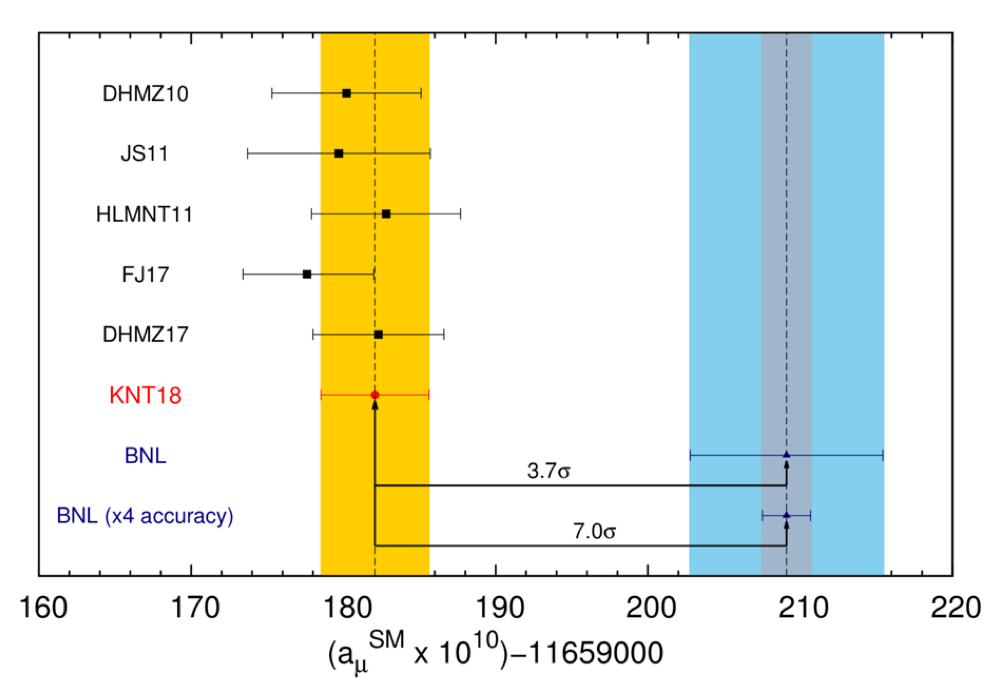
\includegraphics[width=0.9\textwidth]{AlexKPaperComparison}
	\caption[Comparison between theoretical and experimental values for \amu]{Various theoretical values for \amu on the left, as compared to the most recent and extrapolated experimental result on the right. Plot courtesy of Alex Keshavarzi \cite{Keshavarzi:2018mgv}.}
	\label{fig:AlexKPaperComparison}
\end{figure}


\section{Experimental Value of \amu and Discrepancy with \texorpdfstring{$a_{\mu}^{\text{SM}}$}{amusm}}
\label{sec:Background}


The theoretical contributions to \amu listed in the previous sections have improved over time as methods have matured and more experimental data gathered. Similarly, work on the direct experimental measurement of \amu has been going on for decades, with more precise results being determined over time \cite{PastExperiments}. The most recent experiment to measure \gmtwo was the Brookhaven Muon \gmtwo Experiment (E821) held at Brookhaven National Laboratory (BNL) in 2001 \cite{E821FinalReport}. That experiment measured a value for \amu of 
		\begin{align}
            a_{\mu}^{\text{Exp}} = (11659208.0 \pm 6.3) \times 10^{10},
		\end{align}
which corresponds to a 540 ppb relative uncertainty. Note that the uncertainty of the experimental measurement is comparable to that of the theory, necessitating precise understanding of all the different theoretical parts. The difference between the experimental and theoretical values here is
		\begin{align}
            a_{\mu}^{\text{Exp}} - a_{\mu}^{\text{SM}} = (27.74 \pm 7.25) \times 10^{10},
		\end{align}
corresponding to a discrepancy of 3.83$\sigma$ from 0.



-double check the numbers here later on down the line, values like \amu experimental may even have changed if other constants have changed




\section{Beyond the Standard Model and the Purpose of E989}
\label{sec:BSM}


While the discrepancy between experiment and theory might be attributed to miscalculations in the theory or systematic errors in the E821 experiment, no such errors have been found despite serious attempts to resolve the two. Indeed the discrepancy has only grown over time as the theoretical calculations have matured. The most intriguing and exciting source of the discrepancy would be physics beyond the standard model (BSM). Since the value of \amu receives contributions from all particles that couple to the muon through virtual loops, unknown particles might be the source of this discrepancy. Specifically, since the contribution to the magnetic moment from heavy virtual particles goes as 
		\begin{align}
            a \sim \frac{m^{2}}{\Lambda^{2}},
		\end{align}
where $\Lambda$ is the mass scale of the new particle and m the mass of the lepton in question, the senstivity of the muon as compared to the electron to large mass scales is $ m_{\mu}^{2} / m_{e}^{2} \approx 43000$ greater. It is possible from this reason that even though the magnetic moment of the electron has been measured extraordinarily precisely, to .28 parts per trillion (ppt) \cite{ElectronMDM}, it has provided no indication of anything new, whereas the magnetic moment of the muon might provide definitive evidence of new phyiscs.

A basic example diagram of new physics is shown in \figref{fig:BSM}. Because the discrepancy from the previous experiment was not at the 5$\sigma$ level necessary to classify it as a discovery, the E989 experiment was undertaken. Indeed with the lack of new physics results coming out of the LHC and other experiments, E989 is especially positioned to uncover something new at a time where there are so few hints of new physics. Because of this, the interest in the E821 experiment and underway E989 experiment has only grown over time. The number of citations for the E821 results has been consistently high over the years and is shown in \figref{fig:E821Citations}.

\begin{figure}[]
\centering
	\begin{tikzpicture}[baseline=(o.base)]
	\begin{feynhand}
	\large
	\setlength{\feynhandlinesize}{1pt}
	\vertex [ringblob] (o) at (0,0) {BSM};
	\vertex (a) at (-2,-2) {$l$}; 
	\vertex (b) at (2,-2) {$\overline l$}; 
	\vertex (c) at (0,2) {B};
	\propag [fermion] (a) to (o);
	\propag [anti fermion] (b) to (o);
	\propag [photon] (c) to [edge label = $\gamma$] (o);
	\end{feynhand}
	\end{tikzpicture}
\caption[Example diagram for new physics]{An example Feynman diagram, where the leptons couple to an external magnetic field B through some BSM physics. Feynman diagrams made with \cite{tikz-feynman,tikz-feynhand}.}	
\label{fig:BSM}
\end{figure}

\begin{figure}[]
	\centering
	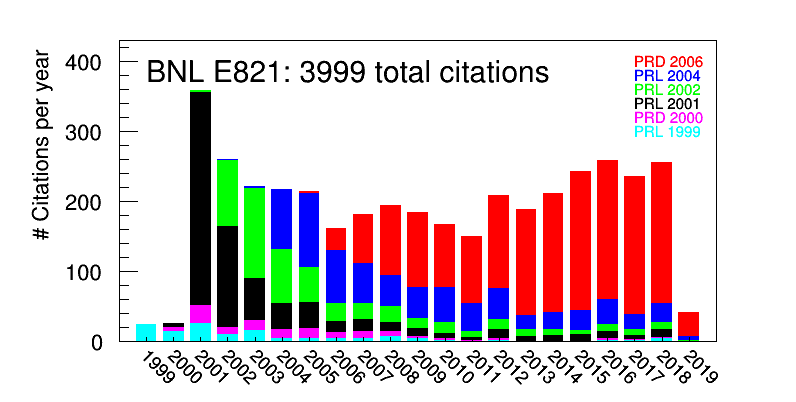
\includegraphics[width=0.9\textwidth]{E821Citations}
	\caption[Citations for E821 publications vs year]{The number of citations for the BNL experiment publications as a function of year. Plot courtesy of Lee Roberts.}
	\label{fig:E821Citations}
\end{figure}


The E989 experiment has the goal of measuring \amu to 140 ppb over the course of several years. This would be a factor of 4 improvement over the E821 result stemming from a 20 times increase in statistics, which was the limiter in the previous experiment. Assuming the same value for \amu is measured, this would push the discrepancy over the 5$\sigma$ mark to approximately 7$\sigma$, as shown in \figref{fig:AlexKPaperComparison}. The data comprising Run 1, gathered in the spring and summer of 2018, is the subject of this thesis, and corresponds to an experimental uncertainty comparable to the E821 result. When it's all said and done, the hope is that we measure something new and exciting, pushing the discrepancy out beyond the 5$\sigma$ level. Even if we do not however, it is valuable in itself to resolve this theoretical and experimental conflict.




% \subsection{Why the muon and not the electron?}

% The magnetic dipole moment of the electron has been measured extraordinarily precisely, to .28 parts per trillion (ppt) \cite{ElectronMDM}. It has been used to test SM theory extensively, and specifically the QED portion of it. Because the electron is so light, the contributions to $a_{e}$ come almost exclusively from QED. This is because the various contributions from both the weak and hadronic sectors contain couplings which depend on the mass of the particle squared. It is for this reason that the magnetic moment of the muon is such an interesting quantity to measure. Since the muon is approximately 200 times heavier than the electron, the senstivity of \amu to radiative corrections is approximately 40000 times greater than that for the the electron.
















